% Options for packages loaded elsewhere
\PassOptionsToPackage{unicode}{hyperref}
\PassOptionsToPackage{hyphens}{url}
%
\documentclass[
]{article}
\usepackage{lmodern}
\usepackage{amssymb,amsmath}
\usepackage{ifxetex,ifluatex}
\ifnum 0\ifxetex 1\fi\ifluatex 1\fi=0 % if pdftex
  \usepackage[T1]{fontenc}
  \usepackage[utf8]{inputenc}
  \usepackage{textcomp} % provide euro and other symbols
\else % if luatex or xetex
  \usepackage{unicode-math}
  \defaultfontfeatures{Scale=MatchLowercase}
  \defaultfontfeatures[\rmfamily]{Ligatures=TeX,Scale=1}
\fi
% Use upquote if available, for straight quotes in verbatim environments
\IfFileExists{upquote.sty}{\usepackage{upquote}}{}
\IfFileExists{microtype.sty}{% use microtype if available
  \usepackage[]{microtype}
  \UseMicrotypeSet[protrusion]{basicmath} % disable protrusion for tt fonts
}{}
\makeatletter
\@ifundefined{KOMAClassName}{% if non-KOMA class
  \IfFileExists{parskip.sty}{%
    \usepackage{parskip}
  }{% else
    \setlength{\parindent}{0pt}
    \setlength{\parskip}{6pt plus 2pt minus 1pt}}
}{% if KOMA class
  \KOMAoptions{parskip=half}}
\makeatother
\usepackage{xcolor}
\IfFileExists{xurl.sty}{\usepackage{xurl}}{} % add URL line breaks if available
\IfFileExists{bookmark.sty}{\usepackage{bookmark}}{\usepackage{hyperref}}
\hypersetup{
  pdftitle={Histopathology Research Template},
  hidelinks,
  pdfcreator={LaTeX via pandoc}}
\urlstyle{same} % disable monospaced font for URLs
\usepackage[margin=1in]{geometry}
\usepackage{color}
\usepackage{fancyvrb}
\newcommand{\VerbBar}{|}
\newcommand{\VERB}{\Verb[commandchars=\\\{\}]}
\DefineVerbatimEnvironment{Highlighting}{Verbatim}{commandchars=\\\{\}}
% Add ',fontsize=\small' for more characters per line
\usepackage{framed}
\definecolor{shadecolor}{RGB}{255,255,255}
\newenvironment{Shaded}{\begin{snugshade}}{\end{snugshade}}
\newcommand{\AlertTok}[1]{\textcolor[rgb]{0.75,0.01,0.01}{\textbf{\colorbox[rgb]{0.97,0.90,0.90}{#1}}}}
\newcommand{\AnnotationTok}[1]{\textcolor[rgb]{0.79,0.38,0.79}{#1}}
\newcommand{\AttributeTok}[1]{\textcolor[rgb]{0.00,0.34,0.68}{#1}}
\newcommand{\BaseNTok}[1]{\textcolor[rgb]{0.69,0.50,0.00}{#1}}
\newcommand{\BuiltInTok}[1]{\textcolor[rgb]{0.39,0.29,0.61}{\textbf{#1}}}
\newcommand{\CharTok}[1]{\textcolor[rgb]{0.57,0.30,0.62}{#1}}
\newcommand{\CommentTok}[1]{\textcolor[rgb]{0.54,0.53,0.53}{#1}}
\newcommand{\CommentVarTok}[1]{\textcolor[rgb]{0.00,0.58,1.00}{#1}}
\newcommand{\ConstantTok}[1]{\textcolor[rgb]{0.67,0.33,0.00}{#1}}
\newcommand{\ControlFlowTok}[1]{\textcolor[rgb]{0.12,0.11,0.11}{\textbf{#1}}}
\newcommand{\DataTypeTok}[1]{\textcolor[rgb]{0.00,0.34,0.68}{#1}}
\newcommand{\DecValTok}[1]{\textcolor[rgb]{0.69,0.50,0.00}{#1}}
\newcommand{\DocumentationTok}[1]{\textcolor[rgb]{0.38,0.47,0.50}{#1}}
\newcommand{\ErrorTok}[1]{\textcolor[rgb]{0.75,0.01,0.01}{\underline{#1}}}
\newcommand{\ExtensionTok}[1]{\textcolor[rgb]{0.00,0.58,1.00}{\textbf{#1}}}
\newcommand{\FloatTok}[1]{\textcolor[rgb]{0.69,0.50,0.00}{#1}}
\newcommand{\FunctionTok}[1]{\textcolor[rgb]{0.39,0.29,0.61}{#1}}
\newcommand{\ImportTok}[1]{\textcolor[rgb]{1.00,0.33,0.00}{#1}}
\newcommand{\InformationTok}[1]{\textcolor[rgb]{0.69,0.50,0.00}{#1}}
\newcommand{\KeywordTok}[1]{\textcolor[rgb]{0.12,0.11,0.11}{\textbf{#1}}}
\newcommand{\NormalTok}[1]{\textcolor[rgb]{0.12,0.11,0.11}{#1}}
\newcommand{\OperatorTok}[1]{\textcolor[rgb]{0.12,0.11,0.11}{#1}}
\newcommand{\OtherTok}[1]{\textcolor[rgb]{0.00,0.43,0.16}{#1}}
\newcommand{\PreprocessorTok}[1]{\textcolor[rgb]{0.00,0.43,0.16}{#1}}
\newcommand{\RegionMarkerTok}[1]{\textcolor[rgb]{0.00,0.34,0.68}{\colorbox[rgb]{0.88,0.91,0.97}{#1}}}
\newcommand{\SpecialCharTok}[1]{\textcolor[rgb]{0.24,0.68,0.91}{#1}}
\newcommand{\SpecialStringTok}[1]{\textcolor[rgb]{1.00,0.33,0.00}{#1}}
\newcommand{\StringTok}[1]{\textcolor[rgb]{0.75,0.01,0.01}{#1}}
\newcommand{\VariableTok}[1]{\textcolor[rgb]{0.00,0.34,0.68}{#1}}
\newcommand{\VerbatimStringTok}[1]{\textcolor[rgb]{0.75,0.01,0.01}{#1}}
\newcommand{\WarningTok}[1]{\textcolor[rgb]{0.75,0.01,0.01}{#1}}
\usepackage{graphicx,grffile}
\makeatletter
\def\maxwidth{\ifdim\Gin@nat@width>\linewidth\linewidth\else\Gin@nat@width\fi}
\def\maxheight{\ifdim\Gin@nat@height>\textheight\textheight\else\Gin@nat@height\fi}
\makeatother
% Scale images if necessary, so that they will not overflow the page
% margins by default, and it is still possible to overwrite the defaults
% using explicit options in \includegraphics[width, height, ...]{}
\setkeys{Gin}{width=\maxwidth,height=\maxheight,keepaspectratio}
% Set default figure placement to htbp
\makeatletter
\def\fps@figure{htbp}
\makeatother
\setlength{\emergencystretch}{3em} % prevent overfull lines
\providecommand{\tightlist}{%
  \setlength{\itemsep}{0pt}\setlength{\parskip}{0pt}}
\setcounter{secnumdepth}{5}
\usepackage{xcolor}
\definecolor{backgroundecho}{HTML}{cccccc}
\definecolor{textecho}{HTML}{333333}

\let\oldverbatim=\verbatim
\let\oldendverbatim=\endverbatim

\makeatletter
\renewenvironment{verbatim}{
    \def\FrameCommand{
        \hskip-\fboxsep
        \color{textecho}
        \colorbox{backgroundecho}
        }
    \MakeFramed{\@setminipage}
    \oldverbatim
}
{
    \oldendverbatim
    \vskip-2em\@minipagefalse % The size required for this negative space is probably in some variable
    \endMakeFramed
}
\makeatother
\usepackage{pdflscape}
\newcommand{\blandscape}{\begin{landscape}}
\newcommand{\elandscape}{\end{landscape}}
\usepackage{xcolor}
\usepackage{afterpage}
\renewcommand{\linethickness}{0.05em}
\usepackage{booktabs}
\usepackage{sectsty} \allsectionsfont{\nohang\centering \emph}
\usepackage{float}
\usepackage{svg}

\title{Histopathology Research Template}
\author{true}
\date{2020-02-26}

\begin{document}
\maketitle

{
\setcounter{tocdepth}{5}
\tableofcontents
}
\begin{center}\rule{0.5\linewidth}{0.5pt}\end{center}

\([![DOI](https://zenodo.org/badge/DOI/10.5281/zenodo.3635430.svg)](https://doi.org/10.5281/zenodo.3635430)\)

\url{https://doi.org/10.5281/zenodo.3635430}

\url{https://osf.io/3tjfk/}

\href{https://sbalci.github.io/histopathology-template/}{Histopathology
Research Template 🔬}

\begin{center}\rule{0.5\linewidth}{0.5pt}\end{center}

\hypertarget{introduction}{%
\section{Introduction}\label{introduction}}

\begin{itemize}
\tightlist
\item
  \textbf{State the marker of interest, the study objectives, and
  hypotheses (Knijn, Simmer, and Nagtegaal 2015)}.\footnote{From Table
    1: Proposed items for reporting histopathology studies.
    Recommendations for reporting histopathology studies: a proposal
    Virchows Arch (2015) 466:611--615 DOI 10.1007/s00428-015-1762-3
    \url{https://www.ncbi.nlm.nih.gov/pmc/articles/PMC4460276/}}
\end{itemize}

\hypertarget{materials-methods}{%
\section{Materials \& Methods}\label{materials-methods}}

\textbf{Describe Materials and Methods as highlighted in (Knijn, Simmer,
and Nagtegaal 2015)}.\footnote{From Table 1: Proposed items for
  reporting histopathology studies. Recommendations for reporting
  histopathology studies: a proposal Virchows Arch (2015) 466:611--615
  DOI 10.1007/s00428-015-1762-3
  \url{https://www.ncbi.nlm.nih.gov/pmc/articles/PMC4460276/}}

\begin{itemize}
\item
  Describe patient characteristics, and inclusion and exclusion criteria
\item
  Describe treatment details
\item
  Describe the type of material used
\item
  Specify how expression of the biomarker was assessed
\item
  Describe the number of independent (blinded) scorers and how they
  scored
\item
  State the method of case selection, study design, origin of the cases,
  and time frame
\item
  Describe the end of the follow-up period and median follow-up time
\item
  Define all clinical endpoints examined
\item
  Specify all applied statistical methods
\item
  Describe how interactions with other clinical/pathological factors
  were analyzed
\end{itemize}

\begin{center}\rule{0.5\linewidth}{0.5pt}\end{center}

\hypertarget{header-codes}{%
\subsection{Header Codes}\label{header-codes}}

\textbf{Codes for general settings.}\footnote{See
  \href{https://github.com/sbalci/histopathology-template/blob/master/childRmd/_01header.Rmd}{\texttt{childRmd/\_01header.Rmd}}
  file for other general settings}

\textbf{Setup global chunk settings}\footnote{Change
  \texttt{echo\ =\ FALSE} to hide codes after knitting and Change
  \texttt{cache\ =\ TRUE} to knit quickly. Change \texttt{error=TRUE} to
  continue rendering while errors are present.}

\begin{Shaded}
\begin{Highlighting}[]
\NormalTok{knitr}\OperatorTok{::}\NormalTok{opts_chunk}\OperatorTok{$}\KeywordTok{set}\NormalTok{(}
    \DataTypeTok{eval =} \OtherTok{TRUE}\NormalTok{,}
    \DataTypeTok{echo =} \OtherTok{TRUE}\NormalTok{,}
    \DataTypeTok{fig.path =}\NormalTok{ here}\OperatorTok{::}\KeywordTok{here}\NormalTok{(}\StringTok{"figs/"}\NormalTok{),}
    \DataTypeTok{message =} \OtherTok{FALSE}\NormalTok{,}
    \DataTypeTok{warning =} \OtherTok{FALSE}\NormalTok{,}
    \DataTypeTok{error =} \OtherTok{TRUE}\NormalTok{,}
    \DataTypeTok{cache =} \OtherTok{TRUE}\NormalTok{,}
    \DataTypeTok{comment =} \OtherTok{NA}\NormalTok{,}
    \DataTypeTok{tidy =} \OtherTok{TRUE}\NormalTok{,}
    \DataTypeTok{fig.width =} \DecValTok{6}\NormalTok{,}
    \DataTypeTok{fig.height =} \DecValTok{4}
\NormalTok{)}
\end{Highlighting}
\end{Shaded}

\begin{Shaded}
\begin{Highlighting}[]
\KeywordTok{library}\NormalTok{(knitr)}
\NormalTok{hook_output =}\StringTok{ }\NormalTok{knit_hooks}\OperatorTok{$}\KeywordTok{get}\NormalTok{(}\StringTok{"output"}\NormalTok{)}
\NormalTok{knit_hooks}\OperatorTok{$}\KeywordTok{set}\NormalTok{(}\DataTypeTok{output =} \ControlFlowTok{function}\NormalTok{(x, options) \{}
    \CommentTok{# this hook is used only when the linewidth option is not NULL}
    \ControlFlowTok{if}\NormalTok{ (}\OperatorTok{!}\KeywordTok{is.null}\NormalTok{(n <-}\StringTok{ }\NormalTok{options}\OperatorTok{$}\NormalTok{linewidth)) \{}
\NormalTok{        x =}\StringTok{ }\NormalTok{knitr}\OperatorTok{:::}\KeywordTok{split_lines}\NormalTok{(x)}
        \CommentTok{# any lines wider than n should be wrapped}
        \ControlFlowTok{if}\NormalTok{ (}\KeywordTok{any}\NormalTok{(}\KeywordTok{nchar}\NormalTok{(x) }\OperatorTok{>}\StringTok{ }\NormalTok{n)) }
\NormalTok{            x =}\StringTok{ }\KeywordTok{strwrap}\NormalTok{(x, }\DataTypeTok{width =}\NormalTok{ n)}
\NormalTok{        x =}\StringTok{ }\KeywordTok{paste}\NormalTok{(x, }\DataTypeTok{collapse =} \StringTok{"}\CharTok{\textbackslash{}n}\StringTok{"}\NormalTok{)}
\NormalTok{    \}}
    \KeywordTok{hook_output}\NormalTok{(x, options)}
\NormalTok{\})}
\end{Highlighting}
\end{Shaded}

\begin{Shaded}
\begin{Highlighting}[]
\NormalTok{  pre}\InformationTok{:not(}\ExtensionTok{[class]}\InformationTok{)}\NormalTok{ \{}
    \KeywordTok{color}\NormalTok{: }\ConstantTok{#333333}\OperatorTok{;}
    \KeywordTok{background-color}\NormalTok{: }\ConstantTok{#cccccc}\OperatorTok{;}
\NormalTok{  \}}
\end{Highlighting}
\end{Shaded}

\textbf{Load Library}

see
\href{https://github.com/sbalci/histopathology-template/blob/master/R/loadLibrary.R}{\texttt{R/loadLibrary.R}}
for the libraries loaded.

\begin{Shaded}
\begin{Highlighting}[]
\KeywordTok{source}\NormalTok{(}\DataTypeTok{file =}\NormalTok{ here}\OperatorTok{::}\KeywordTok{here}\NormalTok{(}\StringTok{"R"}\NormalTok{, }\StringTok{"loadLibrary.R"}\NormalTok{))}
\end{Highlighting}
\end{Shaded}

\begin{center}\rule{0.5\linewidth}{0.5pt}\end{center}

\hypertarget{generate-fake-data}{%
\subsection{Generate Fake Data}\label{generate-fake-data}}

\textbf{Codes for generating fake data}.\footnote{See
  \href{https://github.com/sbalci/histopathology-template/blob/master/childRmd/_02fakeData.Rmd}{\texttt{childRmd/\_02fakeData.Rmd}}
  file for other codes}

\textbf{Generate Fake Data}

This code generates a fake histopathological data. Some sources for fake
data generation here\footnote{Synthea The validity of synthetic clinical
  data: a validation study of a leading synthetic data generator
  (Synthea) using clinical quality measures. BMC Med Inform Decis Mak
  19, 44 (2019) \url{doi:10.1186/s12911-019-0793-0}} , here\footnote{\url{https://bmcmedinformdecismak.biomedcentral.com/articles/10.1186/s12911-019-0793-0}}
, here\footnote{\href{https://synthetichealth.github.io/synthea/}{Synthetic
  Patient Generation}} , here\footnote{\href{https://github.com/synthetichealth/synthea/wiki/Basic-Setup-and-Running}{Basic
  Setup and Running}} , here\footnote{\href{http://www.mli.gmu.edu/index.php/research/ipdg/}{intelligent
  patient data generator (iPDG)}} , here\footnote{\url{https://medium.com/free-code-camp/how-our-test-data-generator-makes-fake-data-look-real-ace01c5bde4a}}
, here\footnote{\url{https://forums.librehealth.io/t/demo-data-generation/203}}
, here\footnote{\url{https://mihin.org/services/patient-generator/}} ,
and here\footnote{lung, cancer, breast datası ile birleştir} .

\textbf{Use
\href{https://github.com/sbalci/histopathology-template/blob/master/R/gc_fake_data.R}{this
code} to generate fake clinicopathologic data}

\begin{Shaded}
\begin{Highlighting}[]
\KeywordTok{source}\NormalTok{(}\DataTypeTok{file =}\NormalTok{ here}\OperatorTok{::}\KeywordTok{here}\NormalTok{(}\StringTok{"R"}\NormalTok{, }\StringTok{"gc_fake_data.R"}\NormalTok{))}
\end{Highlighting}
\end{Shaded}

\begin{Shaded}
\begin{Highlighting}[]
\NormalTok{wakefield}\OperatorTok{::}\KeywordTok{table_heat}\NormalTok{(}\DataTypeTok{x =}\NormalTok{ fakedata, }\DataTypeTok{palette =} \StringTok{"Set1"}\NormalTok{, }\DataTypeTok{flip =} \OtherTok{TRUE}\NormalTok{, }\DataTypeTok{print =} \OtherTok{TRUE}\NormalTok{)}
\end{Highlighting}
\end{Shaded}

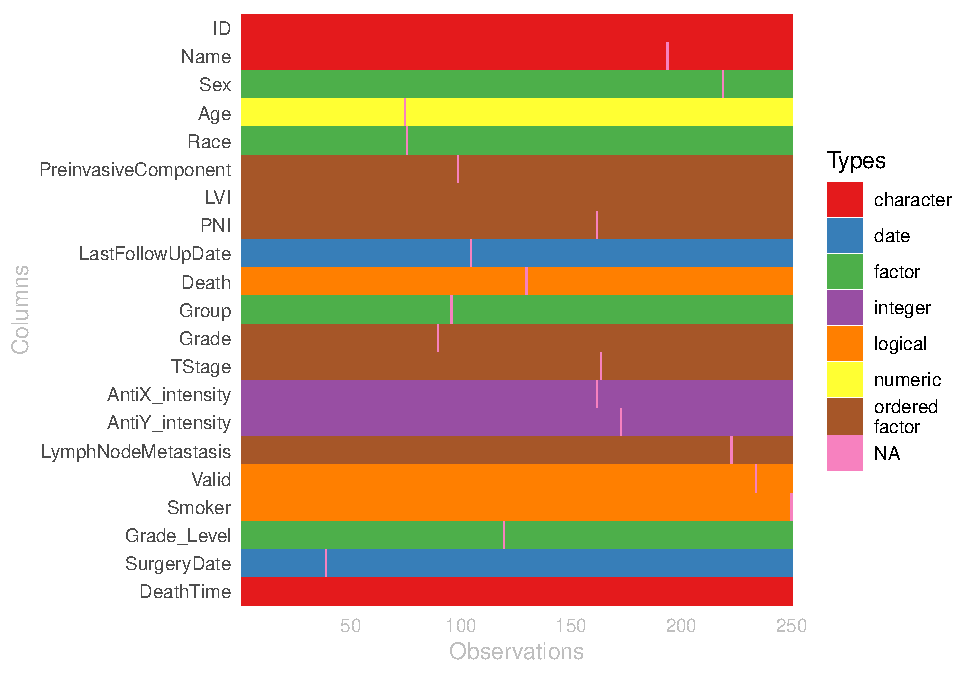
\includegraphics{/Users/serdarbalciold/histopathRprojects/histopathology-template/figs/plot fake data-1.pdf}

\begin{center}\rule{0.5\linewidth}{0.5pt}\end{center}

\hypertarget{import-data}{%
\subsection{Import Data}\label{import-data}}

\textbf{Codes for importing data.}\footnote{See
  \href{https://github.com/sbalci/histopathology-template/blob/master/childRmd/_03importData.Rmd}{\texttt{childRmd/\_03importData.Rmd}}
  file for other codes}

\textbf{Read the data}

\begin{Shaded}
\begin{Highlighting}[]
\KeywordTok{library}\NormalTok{(readxl)}
\NormalTok{mydata <-}\StringTok{ }\NormalTok{readxl}\OperatorTok{::}\KeywordTok{read_excel}\NormalTok{(here}\OperatorTok{::}\KeywordTok{here}\NormalTok{(}\StringTok{"data"}\NormalTok{, }\StringTok{"mydata.xlsx"}\NormalTok{))}
\CommentTok{# View(mydata) # Use to view data after importing}
\end{Highlighting}
\end{Shaded}

Add code for import multiple data purrr reduce

\begin{center}\rule{0.5\linewidth}{0.5pt}\end{center}

\hypertarget{study-population}{%
\subsection{Study Population}\label{study-population}}

\begin{center}\rule{0.5\linewidth}{0.5pt}\end{center}

\hypertarget{ethics-and-irb}{%
\subsection{Ethics and IRB}\label{ethics-and-irb}}

\begin{center}\rule{0.5\linewidth}{0.5pt}\end{center}

\hypertarget{define-variable-types}{%
\subsection{Define Variable Types}\label{define-variable-types}}

\begin{center}\rule{0.5\linewidth}{0.5pt}\end{center}

\hypertarget{overview-the-data}{%
\subsection{Overview the Data}\label{overview-the-data}}

\begin{center}\rule{0.5\linewidth}{0.5pt}\end{center}

\hypertarget{statistical-analysis}{%
\section{Statistical Analysis}\label{statistical-analysis}}

\textbf{Learn these tests as highlighted in (Schmidt et al.
2017).}\footnote{Statistical Literacy Among Academic Pathologists: A
  Survey Study to Gauge Knowledge of Frequently Used Statistical Tests
  Among Trainees and Faculty. Archives of Pathology \& Laboratory
  Medicine: February 2017, Vol. 141, No.~2, pp.~279-287.
  \url{https://doi.org/10.5858/arpa.2016-0200-OA}}

\begin{center}\rule{0.5\linewidth}{0.5pt}\end{center}

\hypertarget{results}{%
\section{Results}\label{results}}

\textbf{Write results as described in (Knijn, Simmer, and Nagtegaal
2015)}\footnote{From Table 1: Proposed items for reporting
  histopathology studies. Recommendations for reporting histopathology
  studies: a proposal Virchows Arch (2015) 466:611--615 DOI
  10.1007/s00428-015-1762-3
  \url{https://www.ncbi.nlm.nih.gov/pmc/articles/PMC4460276/}}

\begin{itemize}
\item
  Describe the number of patients included in the analysis and reason
  for dropout
\item
  Report patient/disease characteristics (including the biomarker of
  interest) with the number of missing values
\item
  Describe the interaction of the biomarker of interest with established
  prognostic variables
\item
  Include at least 90 \% of initial cases included in univariate and
  multivariate analyses
\item
  Report the estimated effect (relative risk/odds ratio, confidence
  interval, and p value) in univariate analysis
\item
  Report the estimated effect (hazard rate/odds ratio, confidence
  interval, and p value) in multivariate analysis
\item
  Report the estimated effects (hazard ratio/odds ratio, confidence
  interval, and p value) of other prognostic factors included in
  multivariate analysis
\end{itemize}

\begin{center}\rule{0.5\linewidth}{0.5pt}\end{center}

\hypertarget{descriptive-statistics}{%
\subsection{Descriptive Statistics}\label{descriptive-statistics}}

\begin{center}\rule{0.5\linewidth}{0.5pt}\end{center}

\newpage
\begin{landscape}

\end{landscape}

\hypertarget{survival-analysis}{%
\subsection{Survival Analysis}\label{survival-analysis}}

\begin{center}\rule{0.5\linewidth}{0.5pt}\end{center}

\begin{center}\rule{0.5\linewidth}{0.5pt}\end{center}

\pagebreak

\hypertarget{discussion}{%
\section{Discussion}\label{discussion}}

\begin{itemize}
\item
  Interpret the results in context of the working hypothesis elaborated
  in the introduction and other relevant studies; include a discussion
  of limitations of the study.
\item
  Discuss potential clinical applications and implications for future
  research
\end{itemize}

\pagebreak

\hypertarget{footer}{%
\section{Footer}\label{footer}}

\begin{center}\rule{0.5\linewidth}{0.5pt}\end{center}

\pagebreak

\hypertarget{references}{%
\section*{References}\label{references}}
\addcontentsline{toc}{section}{References}

\hypertarget{refs}{}
\leavevmode\hypertarget{ref-Knijn2015}{}%
Knijn, N., F. Simmer, and I. D. Nagtegaal. 2015. ``Recommendations for
Reporting Histopathology Studies: A Proposal.'' \emph{Virchows Archiv}
466 (6): 611--15. \url{https://doi.org/10.1007/s00428-015-1762-3}.

\leavevmode\hypertarget{ref-Schmidt2017}{}%
Schmidt, Robert L., Deborah J. Chute, Jorie M. Colbert-Getz, Adolfo
Firpo-Betancourt, Daniel S. James, Julie K. Karp, Douglas C. Miller, et
al. 2017. ``Statistical Literacy Among Academic Pathologists: A Survey
Study to Gauge Knowledge of Frequently Used Statistical Tests Among
Trainees and Faculty.'' \emph{Archives of Pathology \& Laboratory
Medicine} 141 (2): 279--87.
\url{https://doi.org/10.5858/arpa.2016-0200-OA}.

\end{document}
